We next present the results obtained from our experiments using this methodology. We
analyze the number of SLA renegotiations performed by each API consumer during the 112 day
period of the experiment, and calculate a set of cumulative distribution functions (CDF). These
CDFs describe the probability of finding an API consumer that experienced a given number of
renegotiation events. Figure~\ref{fig:renegotiation_cdf} presents the CDFs.

\begin{figure}
\centering
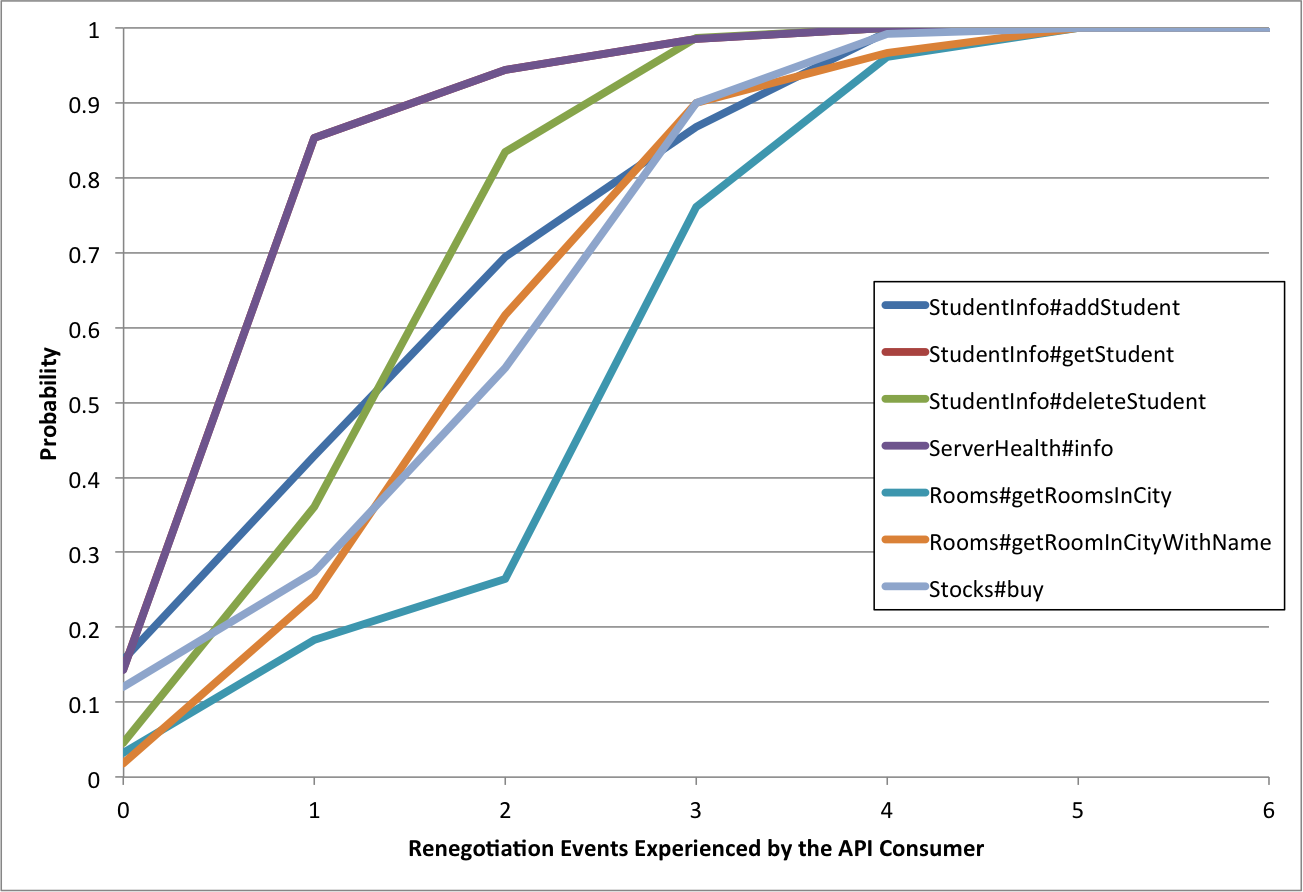
\includegraphics[scale=0.35]{renegotiation_cdf}
\caption{CDF of the number of renegotiation events faced by API consumers.}
\label{fig:renegotiation_cdf}
\vspace{-0.1in}
\end{figure}

According to Figure~\ref{fig:renegotiation_cdf}, the largest number of SLA renegotiations 
experienced by any user is 6. This is
with regard to the StudentInfo\#addStudent operation. Across all web APIs, at least 96\% of the API
consumers experience no more than 4 renegotiation events during the period of 112 days. Further,
at least 76\% of the API consumers see no more than 3 SLA renegotiations, and at least 18\% of
the API consumers observe no more than 1. These statistics
indicate that SLAs predicted by Cerebro for Google App Engine is fairly
stable over time, and renegotiation is required only rarely. From an API consumer's perspective
this is a highly desirable property, since it reduces the frequency and the 
overhead of SLA renegotiation.

Next we analyze the time duration between SLA renegotiation events. For this we combine the SLA validity
periods computed for different API consumers into a single statistical distribution. 
Table~\ref{tab:validity_periods} shows the 5th percentile, mean, and 95th percentile 
of these combined distributions. 

\begin{table}
\begin{center}
\begin{tabular}{|c|p{1cm}|p{1cm}|p{1cm}|}
\hline
Operation & $5^{th}$ & Mean & $95^{th}$ \\ \hline
StudentInfo\#getStudent & 12.97 & 631.24 & 1911.19 \\ \hline
StudentInfo\#deleteStudent & 7.65 & 472.07 & 2031.59 \\ \hline
StudentInfo\#addStudent & 0.05 & 458.24 & 1711.08 \\ \hline
ServerHealth\#info & 12.96 & 630.01 & 1911.19 \\ \hline
Rooms\#getRoomByName & 8.48 & 345.13 & 1096.53 \\ \hline
Rooms\#getRoomsInCity & 20.56 & 296.44 & 1143.45 \\ \hline
Stocks\#buy & 8.46 & 411.75 & 815.5 \\ \hline
\end{tabular}
\end{center}
\caption{Prediction validity period distributions (in hours) of App Engine operations.
$5^{th}$ and $95^{th}$ 
columns represent the 5th and 95th percentiles of the
distributions respectively.
\label{tab:validity_periods}
}
\vspace{-0.3in}
\end{table}

The smallest
mean SLA validity period observed in our experiments is 296.44 hours (12.35 days). This value is given by the
Rooms\#getRoomsInCity operation. 
This implies that on average, API consumers do not have to renegotiate Cerebro-predicted SLAs
for at least 12.35 days.
The smallest 5th percentile value of 0.05 hours is shown by
the StudentInfo\#addStudent operation, but this appears to be a special case compared to the other web API
operations. The second smallest 5th percentile value of 7.65 hours is shown by the 
StudentInfo\#deleteStudent operation. Therefore, ignoring the StudentInfo\#addStudent operation, API
consumers observe SLA validity periods longer than 7.65 hours at least 95\% of the time. That is, the time
between SLA renegotiations is greater than 7.65 hours at least 95\% of the time.

To reduce the number of renegotiations further, we observe that we can exploit the
in which the difference between an invalidated SLA
and a new SLA is small.  In such cases, it is of little use to renegotiate 
a new SLA and API consumers may be content to continue with the old SLA.
To incorporate this behavior into Cerebro (and our simulation process), we introduce threshold
value \textit{sla\_delta\_threshold} into the process. This parameter takes a percentage value that
represents the minimum acceptable percentage difference between the old and new SLA 
values before renegotiation.
If the percentage difference between the two SLA values is below this threshold, we do not record the
SLA validity period, nor increment the count of the SLA invalidations. That is, we do not consider
such cases as renegotiation events. We simply carry on with the
old SLA value until we come across an invalidation event with a percentage difference
that exceeds the threshold. 
Note that our previous experiments are 
a special case of thresholding for which \textit{sla\_delta\_threshold} is 0.

Next we evaluate the sensitivity of our results to the Cerebro \textit{sla\_delta\_threshold}.
Figure~\ref{fig:renegotiation_cdf_sd10}
shows the resulting CDFs of per-user renegotiation count when the threshold is set to 10\%. That is, Cerebro does not prompt the API consumer to renegotiate an SLA, unless the new SLA is at 
least 10\% off from the old one. In this case, the
maximum number of renegotiation events drops from 6 to 5.
Also most of the probabilities shift slightly upwards. For instance,
now more than 82\% of the users see 3 or less renegotiation events (as opposed to 76\%). The
introduction of the \textit{sla\_delta\_threshold} make renegotiations more rare.

\begin{figure}
\centering
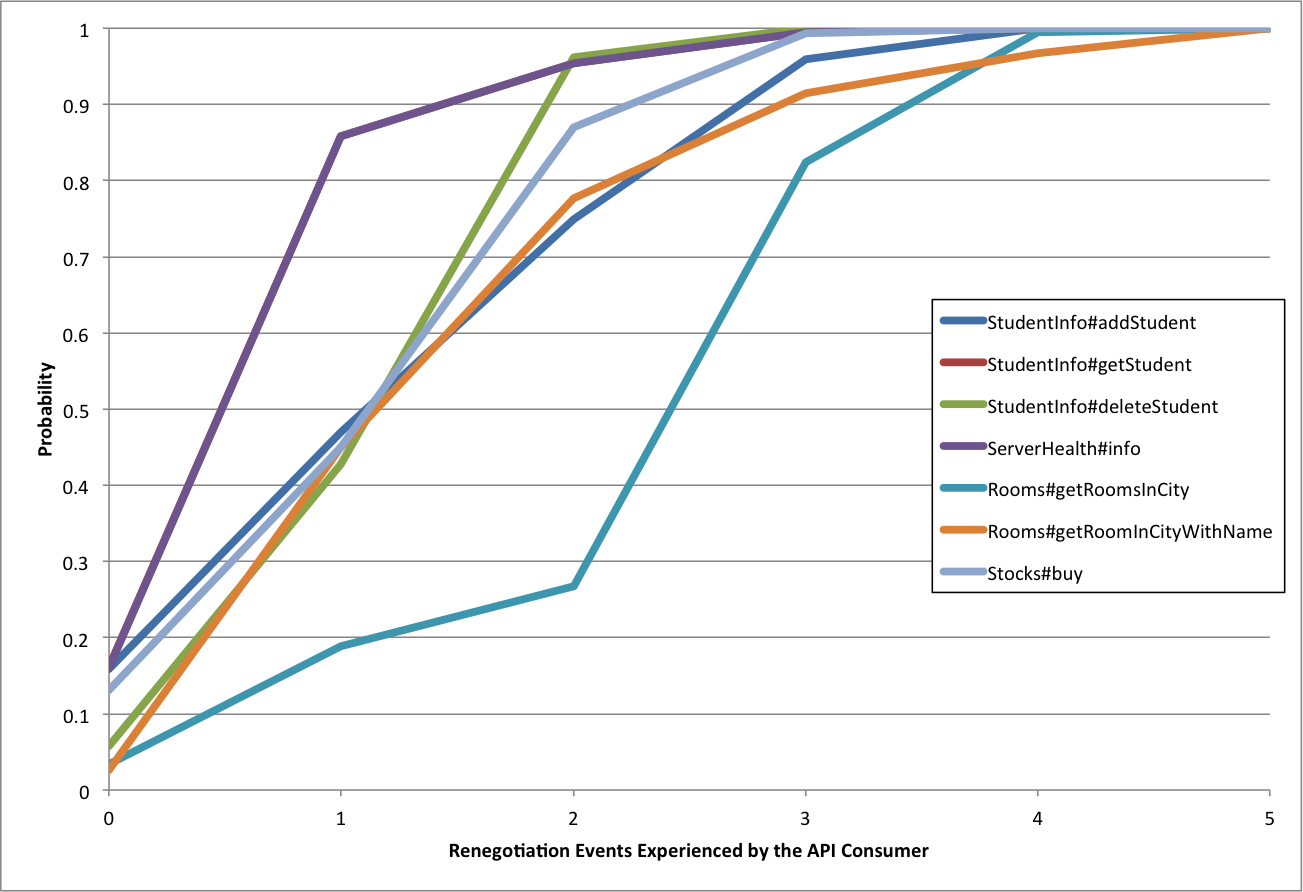
\includegraphics[scale=0.35]{renegotiation_cdf_sd10}
\caption{CDF of the number of renegotiation events faced by API consumers, when  \textit{sla\_delta\_threshold} = 10\%}
\label{fig:renegotiation_cdf_sd10}
\vspace{-0.1in}
\end{figure}

Table~\ref{tab:validity_periods_sd10} shows the SLA validity period distributions computed
when  \textit{sla\_delta\_threshold} is 10\%. Here, as expected  most of the mean and 5th
percentile values have increased slightly from their original values. The smallest mean value
recorded in the table is 304.97 hours. 
We have also considered a \textit{sla\_delta\_threshold} value of 20\%. This change
introduces only small shifts in the probability values of 
the CDFs (more than 84\% of the users see 3 or less renegotiations), 
but the maximum number of renegotiations remains at 5.

\begin{table}
\begin{center}
\begin{tabular}{|c|p{1cm}|p{1cm}|p{1cm}|}
\hline
Operation & $5^{th}$ & Mean & $95^{th}$ \\ \hline
StudentInfo\#getStudent & 19.93 & 644.58 & 1911.19 \\ \hline
StudentInfo\#deleteStudent & 7.93 & 512.52 & 2031.59 \\ \hline
StudentInfo\#addStudent & 0.05 & 491.68 & 1711.08 \\ \hline
ServerHealth\#info & 19.91 & 643.33 & 1911.19 \\ \hline
Rooms\#getRoomByName & 8.48 & 392.01 & 1096.53 \\ \hline
Rooms\#getRoomsInCity & 21.82 & 304.97 & 1143.45 \\ \hline
Stocks\#buy & 7.41 & 510.31 & 1277.7 \\ \hline
\end{tabular}
\end{center}
\caption{Prediction validity period distributions (in hours) of App Engine operations
when \textit{sla\_delta\_threshold} = 10\%. $5^{th}$ and $95^{th}$ 
columns represent the 5th and 95th percentiles of the
distributions respectively. 
\label{tab:validity_periods_sd10}
}
\vspace{-0.3in}
\end{table}


In summary, we find that the performance SLAs predicted by Cerebro 
for the Google App Engine cloud environment are stable over time. That is, the predictions are 
valid for long periods of time, and API consumers need not renegotiate the SLAs 
often. In our experiment spanning over a period of 112
days, the maximum number of renegotiations a user had to undergo was 6. More than 76\% of
the users experienced only 3 or less renegotiations. We can further reduce the number of 
SLA renegotiations per API consumer by introducing a threshold for the minimum applicable
percentage SLA change. This helps to eliminate the cases where an old SLA has been marked as invalid
by our statistical model for detecting SLA invalidations, but the new SLA predicted by Cerebro is not
very different from the old one. However, the effect of this parameter starts to diminish as we
increase its value. In our experiments, we observe the best results for a threshold of
10\%. Using a value of 20\% does not achieve significantly better results.
